%
%   Plantilla propuesta de proyectos
%
%
\documentclass{article} 
\usepackage{ASCIDEN_2024B}
\usepackage{graphicx}
\usepackage{amssymb}
\usepackage{ifthen}
\usepackage{hyperref}
\usepackage[utf8]{inputenc}
\usepackage[spanish]{babel}
\begin{document}
\let\tableline=\hline
\let\obs=\sphericalangle

%%%%%%%%%%%%%%%%%%%%%%%%%%%%%%%%%%%%%%%%%%%%%%%%
% Pagina  1
%%%%%%%%%%%%%%%%%%%%%%%%%%%%%%%%%%%%%%%%%%%%%%%%

% Titulo (debe entrar en una sola linea)

\title {Ingrese aquí el nombre del proyecto.} 


% Abstract
 
\abstract{ 
Escriba aquí un resumen de la propuesta de proyecto. El resumen debe dejar claros los objetivos del proyecto, los datos y metodos a utilizar. 
}

% Informacion de integrantes  

\pinamea{Francisca Hurtado Morales}                  % Nombre
\piinstitutea{Universidad de Chile}        % Institucion
\pigita{FranciscaHM}           % Usuario de GitHub
\piemaila{franbhm04@gmail.com}                 % Direccion de correo

\pinameb{Nombre 2}                  % Nombre
\piinstituteb{Institución 2}        % Institucion
\pigitb{Usuario github 2}           % Usuario de GitHub
\piemailb{Correo 2}                 % Direccion de correo

\pinamec{Nombre 3}                  % Nombre
\piinstitutec{Institución 3}        % Institucion
\pigitc{Usuario github 3}           % Usuario de GitHub
\piemailc{Correo 3}                 % Direccion de correo

\makepgone   % este comando crea la pagina 1




%%%%%%%%%%%%%%%%%%%%%%%%%%%%%%%%%%%%%%%%%%%%%%%%
% Pagina  2
%%%%%%%%%%%%%%%%%%%%%%%%%%%%%%%%%%%%%%%%%%%%%%%%
%
% En esta sección escribe la justificación científica del 
% proyecto. No debe exceder 1 pagina. 
%
\JustificacionCientifica{

Escriba aquí la justificación científica del proyecto. Deben quedar claras las motivaciones del proyecto y lo que se espera obtener de este.

}


\makepgtwo   % este comando crea la pagina 2

%%%%%%%%%%%%%%%%%%%%%%%%%%%%%%%%%%%%%%%%%%%%%%%%
% Pagina  3
%%%%%%%%%%%%%%%%%%%%%%%%%%%%%%%%%%%%%%%%%%%%%%%%
%
% En esta sección escribe la descripción técnica del proyecto
% propuesto. 
% La descripción se divide en dos partes: los datos a
% utilizar y los métodos (o algoritmos) que se explorarán.
% En los métodos, escribe la idea general de los
% procedimientos propuestos. No debe exceder 1 pagina.
%

\datos{

Descripción de los datos a utilizar.

}

\bigskip 

\metodos{

Descripción de los métodos a utilizar.
 
}

\makepgthree % este comando crea la pagina 3

%%%%%%%%%%%%%%%%%%%%%%%%%%%%%%%%%%%%%%%%%%%%%%%%
% Pagina  4
%%%%%%%%%%%%%%%%%%%%%%%%%%%%%%%%%%%%%%%%%%%%%%%%
%
% Usa esta página para agregar referencias y anexos (figuras
% o tablas) que sean de ayuda en la explicación del proyecto
%

\anexos{ 

% Referencias

\References{References}   
Referencias:

\begin{description}       % Agrega tus referencias siguiendo los ejemplos

 \item Hubble, E. P. 1926, ApJ, 64, 321

 \item Penzias, A. A. \& Wilson, R. W. 1965, ApJ, 142, 419 

\end{description}

% Tabla de Ejemplo

\begin{center}
{\bf Tabla 1:} Aca va la leyenda de la tabla. \\
\smallskip
{\small
         \begin{tabular}{lccccr}
            \tableline
            \noalign{\smallskip}
{\rm QSO}&{\rm [Fe/H]}&{\rm [Zn/Fe]}&{\rm [Si/Fe]}&{\rm [S/Fe]}&{\rm Ref.}\\
            \noalign{\smallskip}
            \hline
            \noalign{\smallskip}
Q0149+33   & -1.77  &   0.10  &    0.28 &       ...   &    a,b     \\   
Q0013$-$004& -1.83  &   1.09  &    ...  &       0.79  &    m     \\  

           \noalign{\smallskip}
           \hline

\end{tabular}
}
\end{center}

% Figura de Ejemplo

\center{

   {\bf Figura 1:} Aca va la leyenda de la figura. \\
   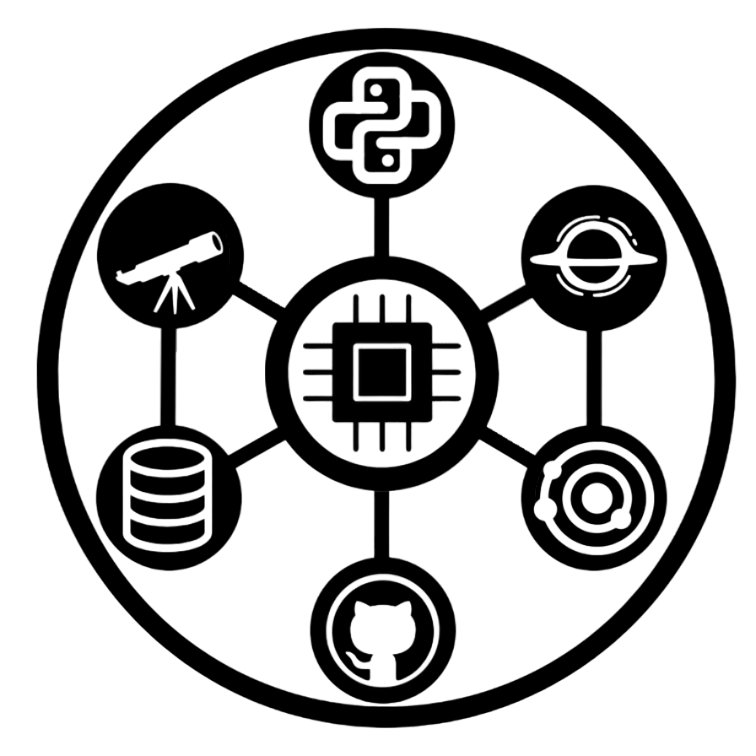
\includegraphics[width=8.5cm,angle=0]{fig1.png}
}


}


\makepgfour   % Este comando crea la pagina 4

\end{document} 

